\documentclass[12pt]{article}

\usepackage[utf8]{inputenc}
\usepackage[english, russian]{babel}

% "А вот теперь --- слайды!"
\usepackage{slides}

\usepackage{array}
\newcolumntype{L}[1]{>{\raggedright\let\newline\\\arraybackslash\hspace{0pt}}m{#1}}

% ШРИФТЫ
% Нужны рубленные шрифты -- раскомментируйте стоку ниже.
% Нужны шрифты с засечками --- закомментируйте эту строку.
% \renewcommand{\familydefault}{\sfdefault} % Переключает на рубленный шрифт.
% Шрифты Times и Arial, если стоит пакет cyrtimes.
\IfFileExists{cyrtimes.sty}
    {
        \usepackage{cyrtimespatched}
    }
    {
        % А если Times нету, то будет CM...
    }

% \renewcommand{\seriesdefault}{b} % для шрифта с засечками, это предпочтительно
% \renewcommand{\seriesdefault}{sbc} % для рубленного шрифта


% Прочие пакетики
% Графика.
\usepackage{graphicx}

% Настройка презентации
% Студент и руководитель.
\def\Student{Стройкова Ксения Александровна}
\def\Advisor{Рогозин Олег Викторович}
% \def\Person
% \def\Affilation
% Титул
\def\Title{Метод сжатия видео на основе кратномасштабного анализа}
% Титул для нижнего колонтитула. Может быть сокращённым
\def\FooterTitle{\Title}
\def\SubTitle{}
\newcommand{\TitleSlide}{
    \addcontentsline{toc}{section}{\Title}%
    ~\vspace{1cm}

    \begin{center}
    {\huge \begin{spacing}{1}\Title\end{spacing}}

    {\SubTitle}
    \vspace{2cm}

    \ifthenelse{\isundefined{\Student}}{}
        {\small Студент: \Student\\}
    \ifthenelse{\isundefined{\Advisor}}{}
        {\small Руководитель: \Advisor\\}
    \ifthenelse{\isundefined{\Person}}{}
        {\Person\\}
    \ifthenelse{\isundefined{\Affilation}}{}
        {\Affilation\\}
    \end{center}
    \thispagestyle{empty}
}


% Верхний заголовок: пустой
% Нижний заголовок по-умолчанию:
% \lfoot{\Title} % слева
% \cfoot{} % цент пуст
% \rfoot{\thepage} % справа

% \renewcommand{\baselinestretch}{1.5}
% \linespread{1.6}


%% Переносы в презентации смотряся не очень.
\hyphenpenalty 10000
\sloppy


\begin{document}

% \raggedright -- грубое выавнивание по левому краю.
% \raggedright

\TitleSlide

% Команды section и subsection начинают новый слайд.

\section{Цель и задачи работы}

\emph{Целью работы} является разработка метода сжатия видео на основе кратномасштабного анализа.

\subsubsection{Решаемые задачи}

\begin{enumerate}
\item Провести анализ существующих методов сжатия видео
\item Разработать метод сжатия видео на основе кратномасштабного анализа
\item Создать приложение, позволяющее применять разработанный метод к видео
\item Разработать модель для оценки предложенного метода
\item Провести исследование работы метода
\end{enumerate}

\section{Сравнение алгоритмов сжатия видео без потерь}

\begin{table}[ht]\footnotesize 
  \begin{tabular}{|p{3.5cm}|p{7cm}|p{7cm}|p{7cm}|}
  \hline
  Алгоритм & Сжатие & Достоинства & Недостатки \\
  \hline
  HuffYUV & каждый кадр, алгоритм Хаффмана & сжатие видео с наличием областей одного цвета на кадрах & не использует избыточность информации между кадрами \\
  \hline
  CorePNG & каждый кадр, алгоритм PNG & наличие прозрачности, возможность гамма коррекции & не использует избыточность информации между кадрами \\
  \hline
  Lagarith & основан на Huffyuv, использует предыдущий кадр при отсутствии изменений & хорошее сжатие при отсутствии движения & не использует избыточность информации между кадрами \\
  \hline
  Motion JPEG 2000 & каждый кадр, алгоритм JPEG 2000 & задается степень сжатия, нет дробления изображения на блоки & сложность алгоритма, не использует избыточность информации между кадрами \\
  \hline
  \end{tabular}
  \label{tab:tabular}
\end{table}  

\section{Сравнение алгоритмов сжатия видео с потерями}

\begin{table}[ht]\footnotesize 
  \begin{tabular}{|p{3.5cm}|p{7cm}|p{7cm}|p{7cm}|}
  \hline
  Алгоритм      & Сжатие & Достоинства & Недостатки \\
  \hline
  M-JPEG  & каждый кадр, алгоритм JPEG & простота реализации & не использует избыточность информации между кадрами, артефакты сжатия \\
  \hline
  MPEG-1       & разбивает кадры по типам, сжимает группы кадров & может использоваться при любом разрешении & поддерживает только прогрессивную развертку \\
  \hline
  MPEG-2   & схож с MPEG-1 & поддерживает видео и в прогрессивной, и в чересстрочной развёртке & требует значительные ресурсы для декомпрессии, плохое качество при малом разрешении видео \\
  \hline
  MPEG-4  & схож с MPEG-1 & улучшен по сравнению с MPEG-1 и MPEG-2 & cтупенчатость при медленном цветовом переходе, артефакты при наличии ошибочных кадров\\
  \hline
  DV  & схож с MJPEG & наложение титров, специальный способ синхронизации аудио и видео информации & специализирован для цифровых камер \\
  \hline
  \end{tabular}
  \label{tab:tabular}
\end{table}

% \section{Сравнение списков}
% 
% Простой текст без списков.
% 
% \begin{itemize}
% \item Список без номеров (\verb+itemize+).
% \item Длинный-предлинный элемент списка с переносом на следующую строку.
% \end{itemize}
% 
% Простой текст без списков.
% 
% Второй абзац простого текста.

% \begin{enumerate}
% \item Пронумерованный список (\verb+enumerate+).
% \item Длинный-предлинный элемент списка с переносом на следующую строку.
% \end{enumerate}

\section{Создание слайда}

\begin{enumerate}
\item Добавление нового слайда: \verb+\section{Заголовок}+.
\item Можно использовать множество команд:
\begin{itemize}
\item нумерованные и ненумерованые списки;
\item формул ($e=mc^2$);
\item моноширный текст (\verb+\section+);
\item разные размеры шрифтов: \scriptsize scriptsize, \tiny tiny, \small small,
\normalsize normalsize, \large large, \Large Large, \LARGE LARGE \normalsize\dots;
\item таблицы и фигуры.
\end{itemize}
\item Latex регулирует интервалы между абзацами и перечислениями для улучшения вида страницы.
\end{enumerate}

\section{Вёрстка слайда в две колонки}

\begin{minipage}[m]{.34\textwidth}
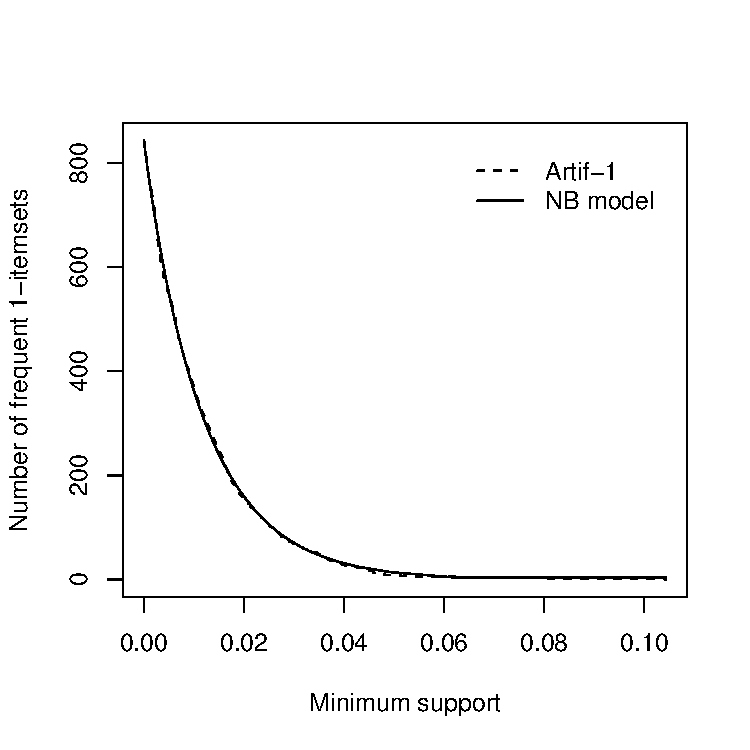
\includegraphics[width=\textwidth]{sample-image}
\centerline{Результаты}
\end{minipage}
%
\begin{minipage}[m]{.65\textwidth}
\raggedright
Для вёрстки отдельных слайдов в две колонки используется окружение
  \verb+minipage+. Здесь использован \verb+\raggedright+ для временного выравнвиания влево.

Пример кода с неравномерными колонками (для равномерных используйте 49 и 49):

\begin{verbatim}
\begin{minipage}[m]{.34\textwidth}
  \includegraphics...
\end{minipage}
\begin{minipage}[m]{.64\textwidth}
  Текст
\end{minipage}
\end{verbatim}

% Недостаток использования \verb+minipage+ --- исчезают интервалы между абзацами.
\end{minipage}

\section{Выводы}

\begin{enumerate}
\item Шаблон презентации в целом отвечает поставленным требованиям.

\item У шаблона в настоящий момент имеются следующие недостатки:
\begin{itemize}
\item при использовании \verb+minipage+ исчезает межабзацный интервал;
\item формулы по-умолчанию несколько меньше текста (при использовании \texttt{cyrtimes});
\item используется выравнивание <<по ширине>>.
\end{itemize}

\end{enumerate}


\end{document}

